\documentclass{article}
\usepackage[utf8]{inputenc}
\usepackage{mathptmx}

\usepackage{color}
\usepackage{graphicx}

\usepackage{amsmath}
\usepackage{amsthm}
\usepackage{amssymb}
\usepackage{braket}
\usepackage{cancel}


% Global formatting macros
\newcommand{\Eqref}[1]{Eq.~(\ref{#1})}
\newcommand{\Comment}[1]{}
\newcommand{\?}{{\color{red}?}}

% Random variables 

%Set theory
\newcommand{\card}{\mathrm {card}}
\newcommand{\Partition}{\mathcal{P}}
\newcommand{\R}{\mathbb R}
\newcommand{\Z}{\mathbb Z}
\newcommand{\N}{\mathbb N}
\newcommand{\chfun}{\mathrm{\chi} }

%Linear space
\newcommand{\Ran}{\mathop{\mathrm{Range}}}

%Arithmetic
\newcommand{\floor}[1]{\lfloor#1\rfloor}
%Vector space
%\renewcommand{\vec}[1]{\underline{#1}}
\newcommand{\tr}{\mathrm{tr}}
\newcommand{\mId}{\mathrm I}

%Vector as list
\newcommand{\len}[1]{|#1|}


% Functionnal analysis
\newcommand{\supp}{\mathop{\mathrm{supp}}}


%Geometry
\newcommand{\Sp}{ \mathcal M}
\newcommand{\Vol}{ \mathrm{Vol}}


% Esperance and statistical quantity
\newcommand{\Esp}[1]{\left<#1\right>}
\newcommand{\Cov}[1]{\mathrm{Cov}_{#1} }
\newcommand{\Var}[1]{\fun{Var}\left[#1 \right]}


%Limits
\newcommand{\conv}[1]{\underset{ #1 \rightarrow +\infty }{\rightarrow} }
\newcommand{\limInf}[1]{\lim_{#1 \rightarrow +\infty}}

% Probability theory notations
\newcommand{\Prob}{P}
\newcommand{\iid}{\mathrm{i.i.d.}}
	%% Convergence type
\newcommand{\as}[1]{\overset{\text{a.s}}{#1}}
	\newcommand{\Dist}[1]{\overset{\mathcal{D}}{#1}}
	\newcommand{\Distas}[1]{\overset{a.s.}{#1}}
	\newcommand{\convD}[1]{\Dist{\conv{#1}} }
	\newcommand{\convas}[1]{\Distas{\conv{#1}} }

	%%Laws
	\newcommand{\lU}{\mathcal U}


% Expression shortcut
\newcommand{\fracpow}[3]{\p{ \frac{#1}{#2}}^{#3}}
\newcommand{\p}[1]{\left(#1\right)} 
\newcommand{\repeated}[2]{ \underbrace{ #1,\dots,#1}_{ #2 \text{ times} } }
\newcommand{\fracLf}[2] { \frac{\Lf\p{#1}}{\Lf\p{#2}} }
\newcommand{\fLf}[1] { \fracLf{#1}{\mE^N} }



% RVMR standard notations
\newcommand{\mE}{\mathcal{E}}
\newcommand{\mP}{\mathcal{P}}
\newcommand{\mR}{\mathcal{R}}
\newcommand{\mA}{\mathcal{A}}
\newcommand{\Lf}{\mathcal{L}}
\newcommand{\mQ}[1]{M(#1)}


% RVMR standard notation for the exemple
\newcommand{\ex}[1]{#1}
\newcommand{\mEx}{ \ex\mE}
\newcommand{\mAx}{ \ex\mA}
\newcommand{\mQx}[1]{\ex{M}\p{#1}}



%Graph theory
\newcommand{\gE}{\mathrm G}
\newcommand{\gtr}{{\mathrm{g}}}
\newcommand{\Conn}{\Pi}


% Article specific notations
	%% Sum 
	\renewcommand{\S}{S}
	%% Immersion
	\newcommand{\Imm}[1]{#1^{\circ}}
	
	%%Jordan Decomposition
	\newcommand{\imJ}{\Imm{J}}

	%%Transition fraction
	\newcommand{\pnu}[1]{\nu_{#1}}

	%%Class decomposition
	\newcommand{\pC}{\mathcal C}
	\newcommand{\pfC}{\overline{\pC}}
	\newcommand{\pdC}{\hat{\pC}}
	\newcommand{\nc}{p}
	\newcommand{\sB}[1]{\Xi_{#1}}
	\newcommand{\sC}[1]{\Xi_{#1}}
	\newcommand{\sdC}[1]{\hat{\Xi}_{#1}}
	\newcommand{\mB}[1]{\mathcal B(#1)}
	\newcommand{\mbP}[1]{\mP^{|#1} }
	\newcommand{\imB}[1]{\Imm{\mathcal B}\p{#1}}


	\newcommand{\fEig}[1]{\rho(#1)}
	\newcommand{\vEig}[1]{\eta(#1)}

	%%Irreducible subchains
	\newcommand{\sPth}[1]{\Gamma^{|#1}}
	\newcommand{\vStat}[1]{ p_{\mathrm{st}}(#1) }
	\newcommand{\bnu}[1]{\nu(#1)}
	\newcommand{\Sq}{c}

	%conditionned quantity
	\newcommand{\cX}[1]{X^{[#1]}}

	%%Structure chain
	% \Delta : structure chain
	\newcommand{\lmax}{{l_{\max}}}

	%t_c upper bound:
	\newcommand{\NcUpB}{\p{\ln N}^2}
	\newcommand{\tcUpB}{ \frac{\NcUpB}{N}}
	\newcommand{\tcUpBl}{ \NcUpB/N }

	%%Reduced model
	\newcommand{\redc}[2][]{#2^{\star#1}}
	\newcommand{\mEr}[1][]{\redc[#1]{\mE}}
	\newcommand{\mPr}[1][]{\redc[#1]{\mP}}
	\newcommand{\mAr}[1][]{\redc[#1]{\mA}}
	\newcommand{\Lfr}[1][]{\redc[#1]{\Lf}}
	\newcommand{\mRr}[1][]{\redc[#1]{\mR}}
	\newcommand{\pthr}[1][]{\redc[#1]{\Gamma}}
        \newcommand{\pCr}[1][]{\redc[#1]{\pC}}

	%%Shadow transition
	\newcommand{\mS}{\theta}
	\newcommand{\mSl}{\Theta}

	%%Periodic chain
	\newcommand{\PGamma}[2]{\sPth{#1,#2}}
	\newcommand{\sPer}[1]{\Theta_{#1}}
	\newcommand{\Pnu}[1]{\nu\p{#1}}

	\newcommand{\fPEig}[1]{\rho(#1)}
	\newcommand{\vPEig}[1]{\eta(#1)}

	\newcommand{\fPtEig}[1]{\rho(#1)}
	\newcommand{\vPtEig}[1]{\eta(#1)}



\begin{document} 
% Random seed used to generate the text file: None
As an example, we consider the following structure matrix $\mEx$ and projection matrix $\mAx$
%
\begin{equation}
\mEx = \begin{pmatrix}
\frac{1}{2}& 1& 0& 1& 0& 0\\[0.1cm]
0& \frac{2}{5}& \frac{3}{5}& 0& 0& 2\\[0.1cm]
0& \frac{1}{4}& \frac{3}{4}& 0& 0& 0\\[0.1cm]
0& 0& 0& \frac{1}{2}& 3& 0\\[0.1cm]
0& 0& 0& 0& \frac{1}{2}& \frac{1}{2}\\[0.1cm]
0& 0& 0& 0& \frac{3}{4}& \frac{1}{4}
\end{pmatrix}, \quad \mAx_{i,j} = 1   
\end{equation}

 
\section{Strongly connected classes $\Xi_i$}
The first step is to identify the irreducible classes (called strongly connected components in graph theory) of $\mE$.
In order to do so, an interesting method is to compute a connectivity matrix $\Conn$
\begin{equation} 
\Conn \equiv \sum_{k=0}^{+\infty} (\epsilon\mE)^k = (\mId- \epsilon\mE )^{-1} .
\end{equation}
For a $\epsilon$ small enough, the matrix $(\mId- \epsilon \mE )$ is diagonal dominant
and therefore easily inversible.
Then, there is a path from $i$ to $j$ if and only if $ \Conn_{ij} >0$.
Applying this algorithm to $\mEx$ and replacing strictly positive coefficients by a symbol $"+"$ yields 
\begin{equation}
%
\ex\Conn = \begin{pmatrix}
+& +& +& +& +& +\\
0& +& +& 0& +& +\\
0& +& +& 0& +& +\\
0& 0& 0& +& +& +\\
0& 0& 0& 0& +& +\\
0& 0& 0& 0& +& +
\end{pmatrix} 
\end{equation}
Once the matrix $\Conn$ has been computed, the next step is to determine a relabelling $i \mapsto i'$
leading to the Perron-Frobenius decomposition.
This relabelling can be found in two steps. First, we identify the strongly connected classes of the graph.
If we call $R(i)_k = \Conn_{ik}$ the $i$th row of the connectivity matrix then two indices $(i,j)$ belong to
the same class if and only if $R(i)=R(j)$:
\begin{equation}
 \{ \sC c \} =  R^{-1}\p{ R \{ 1, \dots, D \} } \;.
\end{equation}
Applying this algorithm to $\Conn$ yields
% 
\begin{equation} %to do correct indices
\{ \ex{\sC{c}} \} =  \Set{\Set{0},\Set{1,2},\Set{3},\Set{4,5}} 
\end{equation}

Finally,  we need to find a ordering $c \mapsto c'$
of these components such that
\begin{equation} \label{eq:clOrder}
i \in \sC{c} , j \in \sC{e} \quad \Conn_{ij} > 0 \implies c' < e' \;.
\end{equation}
A simple way to find this ordering is to start from the set of classes $V_0=\{ \sC{c} \}$.
We can then look at the subset $V_1$ of classes of $V_0$ which have an antecedent among $V_0$.
The difference set $V_0/V_1$ contains the classes which does not have any antecedents classes.
As a consequence, if $\sC{c} \in V_0/V_1$ and $\sC{e} \in V_0$ then we know that $\sC{e} \rightarrow \sC{c}$ is impossible. In other words,
we can safely order the classes of $V_0/V_1$ before the classes of $V_1$ and the ordering of the classes
inside $V_0/V_1$ is arbitrary.  
We can then repeat this procedure by defining $V_{n+1}$ as the subset of classes of $V_n$ with
antecedents among $V_n$:
\begin{equation} \label{eq:app:sseq}
V_{n+1} = \Set{ \Xi  \in V_n | \exists \Xi _e \in V_n/\Xi,\,  \Xi _e \rightarrow  \Xi  }. 
\end{equation}
Note that the cardinal of the set $V_{n+1}$ is always strictly inferior to the cardinal of the set $V_n$
if $V_n$ is not the empty set. Moreover, there cannot be a chain of distinct classes of length greater 
than $\lmax$.  We have therefore $V_\lmax= \emptyset$ and a finite sequence 
\begin{equation}
V_0 \sqsupset V_1 \sqsupset \dots \sqsupset V_\lmax = \emptyset.  
\end{equation}
We can then partition $V_0$ into the difference sets $U_n$
\begin{equation}
  U_n = V_{n+1}/V_n.
\end{equation}
By construction, if $\sC{c} \in U_k$ and $\sC{e} \in U_l$ then 
\begin{equation}
  \label{eq:app:vseq:prop}
  \sC{c} \rightarrow \sC{e} \implies k < l.
\end{equation}
The sequence $U_n$ defines an ordering of the classes $\Set{\sC{c}}$ which is compatible with 
\Eqref{eq:clOrder}. However, this ordering is only a partial ordering of $\Set{\sC{c}}$.
There may be many total orderings of the indices $i$ compatible with this preorder of the classes, but these different 
orderings are equivalent for our purpose. In our example, we have
%% 
\begin{equation} \begin{aligned}
 U_{0} &= \Set{\Set{0}} \\  U_{1} &= \Set{\Set{1,2},\Set{3}} \\  U_{2} &= \Set{\Set{4,5}} \\ 
\end{aligned} \end{equation}
%
Once a specific relabelling has been found, we obtain the Perron-Frobenius form of the matrix $\mEx$
\begin{equation}
\mEx = \begin{pmatrix}
\frac{1}{2}& 1& 0& 1& 0& 0\\[0.1cm]
0& \frac{2}{5}& \frac{3}{5}& 0& 0& 2\\[0.1cm]
0& \frac{1}{4}& \frac{3}{4}& 0& 0& 0\\[0.1cm]
0& 0& 0& \frac{1}{2}& 3& 0\\[0.1cm]
0& 0& 0& 0& \frac{1}{2}& \frac{1}{2}\\[0.1cm]
0& 0& 0& 0& \frac{3}{4}& \frac{1}{4}
\end{pmatrix}
\end{equation}
leading to the following $4$ blocks $\ex{\mB{c}}$: % to do
\begin{equation}
 \mB{1} = \begin{pmatrix}
\frac{1}{2}
\end{pmatrix},\;  \mB{2} = \begin{pmatrix}
\frac{2}{5}& \frac{3}{5}\\
\frac{1}{4}& \frac{3}{4}
\end{pmatrix},\;  \mB{3} = \begin{pmatrix}
\frac{1}{2}
\end{pmatrix},\;  \mB{4} = \begin{pmatrix}
\frac{1}{2}& \frac{1}{2}\\
\frac{3}{4}& \frac{1}{4}
\end{pmatrix},\; 
\end{equation}

\section{ Dominant triplet $\p{\Lambda _c, \vEig c, \fEig c}$}
For each block $\mB{c}$, we have to compute the triplet $\Lambda _c, \vEig c, \fEig c$.
Since the blocks are irreducible by definition, the classical power algorithm
can be used directly. This algorithm consists in computing iteratively a vector $v^{(k)}$:
\begin{equation}
v^{(k+1)} = \frac{ \mB{c} v^{k} } {|| \mB{c} v^{(k)}||},
\end{equation}
starting for an initial vector $v^{0}=1$.
The vector $v^{(k)}$ converges to the dominant right-eigenvector $\vEig c$ when $k \rightarrow \infty$, and the associated eigenvalue $\Lambda _c$ can be computed as
\begin{equation}
\lambda_c^{(k)} =  \frac{ \p{v^{(k)}}^T \mB{c} v_k } { \p{v^{(k)}}^T v^{(k)} } 
\end{equation}
The same algorithm can be used to compute the dominant left-eigenvector of $\mB{c}$
which is the dominant right-eigenvector of $\mB{c}^T$.

Another possibility is to compute the eigenvalue $\Lambda _c$ by using the characteristic polynomial
of $\mB{c}$. This method is generally a little more amenable to symbolic computations.
For instance, in our example, the diagonal blocks of $\ex\mE$ have been 
constructed to be rational multiples of a stochastic matrix. In this very specific case, it is possible to compute exactly
each triplet and obtain
%
\begin{equation} \begin{aligned}
 \lambda_{0} = \frac{1}{2},  \quad& \vEig{0} = \begin{pmatrix}
1
\end{pmatrix}, \quad& \fEig{0} = \begin{pmatrix}
1
\end{pmatrix} \\  \lambda_{1} = 1,  \quad& \vEig{1} = \begin{pmatrix}
1\\
1
\end{pmatrix}, \quad& \fEig{1} = \begin{pmatrix}
\frac{5}{17}\\
\frac{12}{17}
\end{pmatrix} \\  \lambda_{2} = \frac{1}{2},  \quad& \vEig{2} = \begin{pmatrix}
1
\end{pmatrix}, \quad& \fEig{2} = \begin{pmatrix}
1
\end{pmatrix} \\  \lambda_{3} = 1,  \quad& \vEig{3} = \begin{pmatrix}
1\\
1
\end{pmatrix}, \quad& \fEig{3} = \begin{pmatrix}
\frac{3}{5}\\
\frac{2}{5}
\end{pmatrix} \\ 
\end{aligned}\end{equation} 

\section{Limit transition matrix}
%
%
We can then identify the dominant and non-dominant blocks. There is however one caveat
here: if the eigenvalues $\Lambda _c$ are computed using a numerical algorithm, exact comparisons between them
could be meaningless. 
However, the convergence condition for the time $t_c$ spent inside a block $\mB{c}$ gives us a natural comparison between
eigenvalues.
\Eqref{eq:tdist} implies that in order to neglect the time spent inside a block $\mB{c}$, we need to verify that
\begin{equation} \label{eq:neglect}
\fracpow{\Lambda _c}{\Lambda }{n} \gg 1.
\end{equation}
Consequently, \Eqref{eq:neglect} defines a sensible criterion for the comparison between $\Lambda _c$'s.  
With this caveat in mind, we can construct the limit transition matrix $\mS$ from the normalized
structure matrix $\mE/\Lambda $.
\begin{equation}
 \mSl = \sum _{k=0}^{+\infty } \mS^{k} = \p{\mId - \mS }^{-1} \;,
\end{equation}
where $\theta$ is defined in \Eqref{eq:shw}.
In our example,
\begin{equation}
\ex\mSl = \begin{pmatrix}
2& 2& 0& 4& 12& 4\\[0.1cm]
0& 1& 0& 0& 0& 2\\[0.1cm]
0& 0& 1& 0& 0& 0\\[0.1cm]
0& 0& 0& 2& 6& 0\\[0.1cm]
0& 0& 0& 0& 1& 0\\[0.1cm]
0& 0& 0& 0& 0& 1
\end{pmatrix}.
\end{equation}

\section{Reduced model}
With this, we have obtained all the information needed 
to compute $\p{\mEr,\mAr,\mPr}$ using Eqs.~(\ref{eq:Er}), (\ref{eq:Ar}) and~(\ref{eq:Pr}).
Here, we have for $\ex\mAr$ and $\ex\mEr$
%
\begin{equation}
\ex\mAr= \begin{pmatrix}
\frac{108}{17}& \frac{54}{17}\\
0& \frac{284}{5}
\end{pmatrix} ,\quad  \ex\mEr = \begin{pmatrix}
1& \frac{4}{5}\\[0.1cm]
0& 1
\end{pmatrix}
\end{equation}
We can also determine the path of maximal length, which is unique here, and its probability,

\begin{equation} \begin{aligned}
 \pC_{1} =\Set{0,1}, \quad &p\p{\pC_{1}} =1 %
\end{aligned} \end{equation} 
\section{Limit laws for the central limit theorem}

Once we know the triplet $(\mEr,\mAr,\mPr)$ and the maximal path $\pC $, it is possible to compute the limit distribution
for the central limit theorem using \Eqref{eq:lim:CLT2}. 
If we suppose that the moment matrix $\mQ{1}$ has all its coefficients identical, namely $\mQ{1}_{ij}= \mu$, it is possible to use \Eqref{eq:lim:CLT2}
to compute the limit distribution of the centered variable $z = (S(\vec X) - N\mu )/ \sqrt{N}$.
On the one hand, it does not seem possible to obtain an explicit analytic form for the integral~\eqref{eq:lim:CLT2}.
On the other hand, its form is quite convenient for a Markov integration.
The only difficulty is the presence of the Dirac distribution $\delta(1 - \sum_i \alpha_i )$.
However, in terms of Markov integrals, this distribution corresponds to a uniform sampling of the $\alpha_i$ on the $(\lmax-1)$-simplex
\begin{equation}
\Sp_\pC = \{ \alpha,\quad \forall i ,  \alpha_i >0,\, \sum_{i=1}^{\len{\pC } } \alpha_{\pC _i}=1 \}. 
\end{equation}
Moreover, sampling uniformly on a $\lmax$-simplex can be done by generating $\lmax$
$\iid$ exponential random variables with the same shape parameter and then normalize (accordingly to the $||\cdot ||_1$ norm) the
resulting vector. Fig.~\ref{fig:clt} illustrates the limit law for our example if we choose
the following variance for the reduced model 
\begin{equation}
\sigma^{2}_{ii} = \p{\frac{70}{51}}.
\end{equation}
%
\begin{figure}
\centerline{ 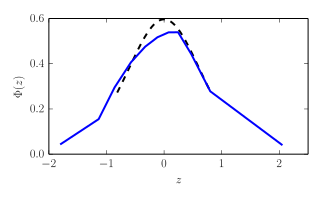
\includegraphics[width=0.7\columnwidth]{Figs/CLT} }
\caption{ \label{fig:clt} Limit law for the centered variable $z=(S-N\mu)/\sqrt{N}$ computed with a Markov integral method. Dashed black line: theoretical distribution; Blue line:
empirical histogram computed from $1000$ realizations of $\vec X$ with $N=500$.}
\end{figure}



\section{Limit distribution for the law of large numbers} \label{sec:geom}
In order to determine explicitly the limit distribution for the sample mean $s=S(\vec X)/N$ for a given structure path $\pC $, we have to evaluate 
the integral~\eqref{eq:lim:LLN2}. There are two essential differences with the case of the central limit theorem. 
First, there is one more Dirac distribution
$\delta \p{ s - \sum _k \alpha _k  \mu _{\pC_k \pC_k} }$. This implies that the integral~\eqref{eq:lim:LLN2} is null except on the manifold
\begin{equation}
K_{\pC }(s) = \Sp_{\pC } \cap H_{\pC }(s) \;,
\end{equation}
with $H_{\pC }(s)$ the hyperplane
\begin{align}
H_{\pC }(s) = \{ \alpha  \in  \R ^{\lmax} | \sum _k \alpha _k \mu _{\pC _k \pC _k} = s \}.
\end{align}
$\Sp_{\pC }$ is the standard $(\lmax-1)$-simplex and enforces the condition that 
the sum of the $\alpha _i$'s is equal to $1$, whereas $H_\pC (s)$ is the set of $\alpha $ corresponding to an average $s$.
Second, except for the Dirac distribution the integral does not contain any varying term.
Consequently, if we restrain the integration domain of \Eqref{eq:lim:LLN2} to the support of the Dirac distribution, we have
\begin{equation} \label{eq:pregeom}
 p \p{ \frac{S(\vec X | \pC )}{n} = s }  = \frac{1}{V}\int_{K_\pC (s)} 1 d\alpha ,
\end{equation}
with $V$ a normalization constant.
The constant integral in \Eqref{eq:pregeom} can be interpreted as a measure of the 
volume of the manifold $K_\pC (s)$:
 \begin{equation} \label{eq:lln:geom}
 p \p{ \frac{S(\vec X | \pC )}{n} = s } = \Vol \p{K_\pC (s)}.
\end{equation}
Computing the volume of a general manifold can be quite difficult. However, $K_\pC (s)$
can be decomposed as an intersection of half-spaces and hyperplanes. It is thus a convex polytope,
a very specific subset of manifold which has been studied extensively. In particular, in order 
to compute the volume of a polytope a standard method consists in dividing the polytope into
a collection of simplices (i.e generalized triangles). For a given simplex $s$ with vertices $\{ v_1, \dots, v_k \}$ its volume can be computed by 
\begin{equation}
\Vol(s) = \det\p{v_2-v_1, \dots, v_k - v_1}.
\end{equation}
The volume of the whole polytope is then the sum of the volume of its decomposition in elementary simplices.
An interesting consequence of this is that the total volume of $K_\pC (s)$ depends only on the vertices of the polytope 
$K_\pC (s)$. As $K_\pC (s)$ is the intersection of $\Sp_{\pC }$ and the hyperplane $H_\pC (s)$, these vertices correspond 
to the intersection of the edges of $\Sp_{\pC }$ and the hyperplane $H_\pC (s)$. If we call $e_1,\dots,e_{D}$ the canonical
base of $\R^D$, the vertices of $\Sp_{\pC }$ are $e_{\pC _1},\dots, e_{\pC _{\lmax}}$. Then any $[e_{\pC _k}, e_{\pC _l}]$ segment is an edge of $\Sp_{\pC }$.
These segments are intersected by $H_\pC (s)$ if and only if their two end points lay on different sides of $H_\pC (s)$.
At a global level, if there are $k$ vertices on one side of $H_\pC (s)$ and $l$ on the other side, then $K_\pC (s)$ will
have $kl$ vertices. For instance, in dimension 4, the hyperplane $H_\pC (s)$ separates the $4$-simplex in either a $(1,4)$ 
configuration or a $(2,3)$ configuration. The first $(1,4)$ configuration corresponds to a tetrahedron with $4$ vertices.
The other $(2,3)$ configuration is a distorted triangular prism with $6$ vertices. In arbitrary dimension,
$K_\pC (s)$ is a kind of generalized prism\footnote{More precisely $K_\pC (s)$ is diffeomorph 
to the cartesian product of a $|l-1|$-simplex and a $|r-1|$-simplex.}. 
The important result here is that the shape of $K_\pC (s)$ only changes when $H_\pC (s)$ crosses one of the $e_{\pC _k}$ vertices.
If we call $s^{\wedge}_t$ these crossing points, then on the intervals $(s^{\wedge}_t,s^{\wedge}_{t+1})$, the vertices $v_{k,l}$ of
$K_\pC (s)$ are affine functions of $s$ 
\begin{equation}
v^{k,l}(s) =  \frac{ s -  \mu _{ll} }{ \mu_{kk} - \mu _{ll} }  e_k + \frac{ s - \mu _{kk} }{ \mu _{ll} - \mu _{kk} }  e_l. 
\end{equation} 
Consequently, on the interval $(s^{\wedge}_t,s^{\wedge}_{t+1})$, $\Vol(K_\pC (s))$ is a polynomial function.
Hence, the limit distribution for the law of large numbers is a piecewise polynomial.
Moreover, it is possible to use symbolic computation to compute exactly the limit distribution from the means $\mu_{i,i}$. For instance, if we arbitrarily choose 
\begin{equation}
\mu_{ii} = \p{\frac{684}{221}}.
\end{equation}
for our example, we have
%
\begin{equation}
 p \p{ \frac{S(\vec{X})}{N} = s } = \begin{cases}
 0 & s \in (-\infty,99/170)\\
\frac{2210}{5553} & s \in [99/170,684/221)\\
 0 & s \in [684/221, +\infty )
 \end{cases} 
\end{equation}
%


\begin{figure}
\centerline{ 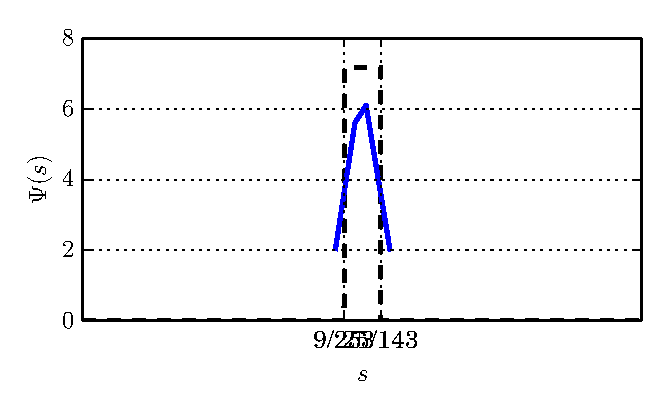
\includegraphics[width=0.7\columnwidth]{Figs/LLN} }
\caption{ \label{fig:lln} Limit law for sample average $s=S/N$ computed using a geometric method.
Dashed black line: theoretical distribution; Full blue line:
empirical histogram computed from $1000$ realizations of $\vec X$ with $N=500$.
Dotted red line: angular points of the theoretical limit distribution. 
}
\end{figure}

\end{document}

